\section{Steps}

\subsection{Einbinden von Nuitrack}
Nuitrack kann unter folgendem Link für alle Platformen runtergeladen werden: \href{https://github.com/3DiVi/nuitrack-sdk/blob/master/doc/Install.md} .

\subsubsection{Import Nuitrack Wrapper in Unity}
Unter folgendem git repo kann das Nuitrack Plugin runtergeladen werden: \href{https://github.com/3DiVi/nuitrack-sdk/blob/master/Unity3D/NuitrackSDK.unitypackage} . Da dieses Plugin für verschiede Sensoren, also Kameras konfiguriert wurde, muss dann noch der Sensor spezifiziert werden. In meinem Projekt ist dies die IntelRealsense D435.


\subsubsection{Skeleton Tracking mit NuitrackSDK}
Das Tutorial von Nuitrack ist meine Ausgangslage um eine Person zu tracken. Der Link führt zu diesem Tutorial: \href{https://github.com/3DiVi/nuitrack-sdk/blob/master/doc/Unity_Face_Tracking.md} .

\subsection{Virtuelle Szene in Unity}
In Unity baue ich die Szene so auf, dass die Render-Kamera in positiver z-Achse ausgerichtet ist. Anfangsposition der Render-Kamera ist (0, 0.2, -1.5). Den Screen welcher dann entzerrt werden soll, setze ich auf den Nullpunkt. Also genauer die Mitte vom Screen hat die Position (0, 0, 0).
Die Eckpunkte vom Screen haben die folgenden Positionen: 
P0(-0.8, -0.45)
P1( 0.8, -0.45)
P2( 0.8,  0.45)
P3(-0.8,  0.45)
Der Screen hat die Grösse 1600 x 900 mm. Dieser wird als schmaler Kubus dargestellt und transparent leicht grau eingefärbt, damit ich dann erkannen kann ob mein Rendern und Entzerren richtig funktioniert.
Die Main-Kamera setze ich als Referenz auf die Position der Render-Kamera. Dies damit ich eine Ansicht in der Szene bekomme. Die Main-Kamera zeigt dann die Szene und für den Output vom entzerrten Screen benötige ich das gerenderte Bildmaterial der Renderkamera. 
Gut möglich, dass man dies auch mit weniger Kameras darstellen kann.

\subsubsection{Render Kamera zeigt Position vom Betrachter}
Die Render-Kamera wird als Referenz auf den obersten Knochen vom Skelett gemappt. Dieser oberste Knochen entspricht dem Kopf, genauer der Stirn.
Damit wird dann auch die Main-Kamera, welche die Render-Kamera referenziert auf den Kopf gemappt.

\subsubsection{Render Kamera zeigt RenderTexture}
Die Render-Kamera wird nun stets auf den Mittelpunkt vom Screen gerichtet. Der Output der Render-Kamera erzeugt dann eine RenderTexture der Grösse 750 x 750 Pixel. Je grösser die Anzahl Pixel, desto besser wird dann die Qualität vom Endbild.

\subsection{Matrix Shader}
Im Netz habe ich einen Rotations Shader gefunden und versucht diesen so anzupassen, dass die Entzerrung gelingt. Leider ohne Erfolg. Das Probelm bei diesem Shader funktioniert das Scaling und das Shearing, nicht aber die Translation. Zudem wüsste ich nicht, wie ich mit dieser Rotationsmatrix das Polygon selektieren sollte.
Als Einstieg in die Unity Shader hat es trotzdem etwas geholfen, mehr aber auch nicht.

\subsection{Pixel Shader}
Damit ich diese Entzerrung vom Polygon machen kann, benötige ich einen Pixel-Shader. Oder einen Shader welcher die Maintexture ändert.
So habe ich nun einen Shader welche als Parameter die Maintextur als Eingabewert hat. Im Script wird dann in der Update Funktion für jedes Pixel der Farbwert gesetzt und am Ende die Textur dem Shader übergeben.

\subsection{Entzerrung vom Polygon}
\subsubsection{Homographie}
Zuerst habe ich versucht die Entzerrung mit einer Homographie Matrix zu erreichen. Leider hat dies nur geklappt für die Ansicht ohne seitliche Verschiebung, also mit einem x-Wert von Null. Sobald ich etwas abweiche von dieser zentralen Position, zeigt sich ein Shearing im Output Bild, welches sich auch noch anders verhält, je nachdem ich in positiver x-Achse gehe oder in negativer x-Achse. 
Ich habe da länger darüber nachgedacht, meine Homographie Matrix mehrmals geprüft, fand aber nicht heraus was das Problem war. Komisch ja auch, dass es in zentraler Position den Richtigen Output gab, bei seitlicher Verschiebung sich dann aber ein Shearing zeigt, welches mit grösserer Abweichung nach links oder rechts dann auch noch grösser wurde.
Somit brauche ich einen anderen Ansatz um die Entzerrung zu lösen.

\subsubsection{OpenCV}
OpenCV hat bereits Methoden, welche diese Entzerrung vornehmen. Das Plugin von OpenCV findet sich unter: \href{https://github.com/EnoxSoftware/OpenCVForUnity/tree/master/Assets/OpenCVForUnity} .
Die grösste Schwierigkeit ist bei OpenCV, dass Unity einen anderen Aufbau der Matrizen hat und dass OpenCV keine Textures kennt. 
Die grösste Schwierigkeit war dann zu merken, dass die Pixelwerte der Textures in OpenCV nicht einfach so auf der CPU verfügbar sind. Diese werden auf der GPU gespeichert und mössen dann exklusiv abgefragt werden.
Die Funktionen von OpenCV funktionieren tadellos. Damit die Entzerrung gelingt, gehe ich vom Zielbild aus und berechne die Perspektivische Matrix rückwärts vom Zielbild zum Inputbild, was dann dem Inversen der Perspektivischen Matrix entspricht. 
Nun wird diese Matrix auf jedes Pixel des Zielbildes angewendet und so den Farbwert an der entsprechenden Stelle im Inputbild geholt. 
Da diese Operation mit der Anzahl Pixel steigt, habe ich hier ein Format vom Zielbild 800 x 450 Pixel gewählt.

\subsection{Berechnung der Polygon Eckpunkte}
\subsubsection{Kameramodell}
Ich habe versucht mittels Kameramodell die Transformationsmatrix für die Eckpunkte vom Screen zu berechnen. Dazu braucht man den Viewport, die intrinsiche (Projektionsmatrix) und die extrinsische Kameramatrix (Viewmatrix). Da sich der Screen nicht verschiebt, braucht es die Modellmatrix nicht.
 
\subsubsection{Projektion der Eckpunkte auf der Zielebene}
Mein Ansatz den ich umgesetzt habe funktioniert wie folgt: 
Unity hat eine Funktion welche mir die Eckpunkte von der Clipping Ebene entsprechend dem z Wert herausscheibt. Ich wähle diese Ebene durch den Nullpunkt, auf welchen sich die Render-Kamera immer richtet. 
Nun projeziere ich die Eckpunkte vom Screen in der Verlängerung von der Render-Kamera durch die Eckpunkte. Die Schnittpunkte mit der Ebene müssen nun nur noch relativ zu den Ecken der Clipping Ebene berechnet werden. 

\subsection{FaceManager}
{
	\thicklines
	% \thinlines
	\lstinputlisting[style=bfh-c,language={[Sharp]C},caption={FaceManager},label={FaceManager}]{listings/FaceManager.cs}
}
Erklärungen zum Script FaceManager listing~\ref{FaceManager}


\subsection{PixelAlgoScript}

{
	\thicklines
	% \thinlines
	\lstinputlisting[style=bfh-c,language={[Sharp]C},caption={PixelAlgoScript},label={PixelAlgoScript}]{listings/PixelAlgoScript.cs}
}
Erklärungen zum PixelalgoScript listing~\ref{PixelAlgoScript}

\subsection{PixelShader} 
\begin{figure}[hbt!]
	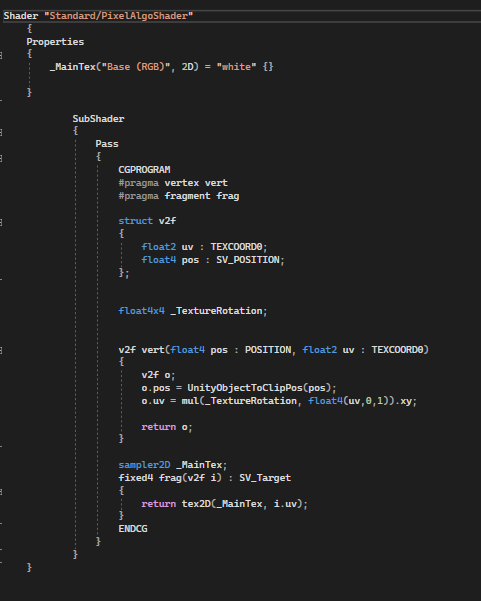
\includegraphics[width=1.0\linewidth]{PixelAlgoShader}
	\caption{PixelShader in Unity}
\end{figure}



